\documentclass[a4paper,11pt,fleqn]{scrartcl}%fleqn pour aligner les equations à gauche
\usepackage{../../Styles/Cours}


\newcommand{\chnum}{Chapitre 13}
\newcommand{\chtitle}{Influence du poids}
\newcommand{\dtype}{TP}

\begin{document}
	\maketitle
    Certaines compagnies aériennes choisissent de ne pas appliquer de peinture sur leurs avions ce qui leur permet de réduire leur masse de manière considérable.\\

    \noindent\begin{minipage}{\linewidth}
    \begin{documentboxenv}{Le dispositif expérimental}
        \label{doc1}
        Le Smart Cart PASCO, muni de capteurs connectés, enregistre ses positions à intervalles de temps réguliers et les transmets au logiciel de traitement Capstone. Tous les frottements sont négligés.
        \begin{center}
            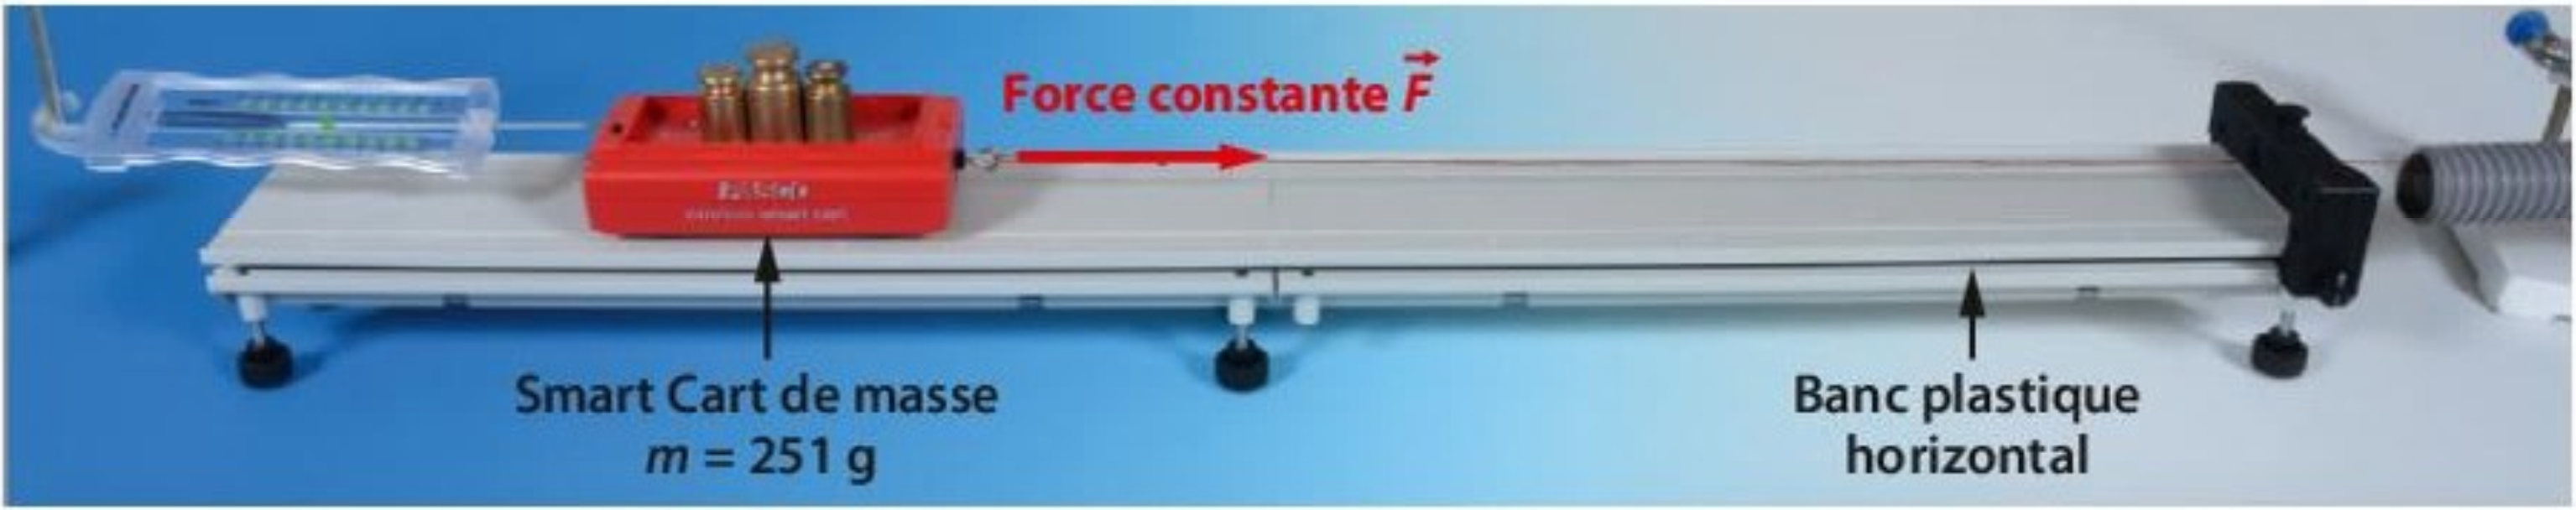
\includegraphics[width=.8\linewidth]{Ressources/PASCO_Smart_Cart.png}
        \end{center}
    \end{documentboxenv}
    \end{minipage}
    
    \begin{minipage}{.49\linewidth}
        \begin{documentboxenv}{Smart Cart tiré par une force constante $F =\SI{0,7}{\newton}$}
        \label{doc2}
        \begin{center}
            \begin{tabular}{|>{\centering}m{5em}|c|c|c|c|c|}
                \hline
                Masse marquée $M$ \unit{g} & 300 & 400 & 500 & 600 & 700 \\
                \hline
                Masse totale $m$ \unit{kg} &  &  &  &  &  \\
                \hline
                Vitesse atteinte à \SI{200}{\milli\second} \unit{\meter\per\second} & 0,40 & 0,34 & 0,32 & 0,31 & 0,28 \\
                \hline
                Vitesse atteinte à \SI{500}{\milli\second} \unit{\meter\per\second} & 0,81 & 0,68 & 0,59 & 0,56 & 0,51 \\
                \hline
                $\Delta v$ (\unit{\meter\per\second}) &  &  &  &  &  \\
                \hline
                $\dfrac{\Delta v}{\Delta t}$ (\unit{\meter\per\second\squared}) &  &  &  &  &  \\
                \hline
            \end{tabular}
        \end{center}
        La patineuse est assomilée à un point matériel. Ses positions successives sont données à l'intervalle de temps $\tau = \SI{40}{\milli\second}$.
        \end{documentboxenv}
    \end{minipage}
    \begin{minipage}{.49\linewidth}
        \begin{documentboxenv}{Programme Python influenceMasse.py à compléter}
        \label{doc3}
        \begin{center}
            \lstinputlisting[language=Python]{influenceMasse.py}
        \end{center}
        La patineuse est assomilée à un point matériel. Ses positions successives sont données à l'intervalle de temps $\tau = \SI{40}{\milli\second}$.
        \end{documentboxenv}
    \end{minipage}

    \begin{question}
        \begin{enumerate}
            \item Définir le système étudié et le référentiel choisi pour décrire les mouvements.
            \item Faire le bilan des actions mécaniques exercées sur le système et déterminer le vecteur $\sum \vv{Forces}$.
            \item Ouvrir et compléter le fichier Python influenceMasse.py (Doc.~\ref{doc3}) pour calculer la masse totale $m$ du Smart Cart en fonction de la masse marquée $M$ et compléter le tableau du Doc. 2 en exécutant le programme.
            \item Décrire à l'aide de vos résultats comment la masse de peinture d'un avion influe sur la variation de la vitesse entre deux instants voisins.
            \item Indiquer les grandeurs à porter en abscisses et en ordonnées pour tester la relation approchée $F \approx m_{systeme} \times \dfrac{\Delta v}{\Delta t}$ et pouvoir la modéliser par une droite.
        \end{enumerate}
    \end{question}
\end{document}